% intro.tex
% --------------------------------------------------------------------------

Polygonal boundary representations in computer graphics are typically
implemented with one of the edge-centered data structures for meshes,
such as; doubly-connected edge list, winged-edge, quad-edge, or
halfedge data structure. Common practice is to develop such data
structure from scratch, since clearly a first implementation is at the
level of a students homework assignment. But then, these data
structures consist almost entirely of pointers for all sort of
incidence informations. Maintaining them consistently during mesh
operations is not anymore a trivial linked-list update operation. So,
moving from a students exercise to a reliable research implementation
, including maintaining and optimizing such an implementation, is a
respectable software task.
%, just imagine to introduce a back-pointer for
%an existing incidence pointer and change all operations on the mesh to
%handle this additional pointer consistently.

What is common practice for simple data structures, such as linked
lists, should be common practice even more so for mesh data
structures, namely, to use a good, flexible, and efficient library
implementation. In \CC\, the \emph{Standard Template Library}, \stl,
is an excellent address for our analog example of the linked lists,
and we argue in this paper that an excellent flexible mesh data
structure together with a rich and versatile infrastructure for mesh
algorithms exists in the \emph{Computational Geometry Algorithms Library},
\cgal~\footnote{\path|http://www.cgal.org/|}.

We will review the design of the polygonal boundary representation
\cgalpoly\ in \cgal\ that is based on the halfedge data structure.
Our main new contribution is \emph{a tutorial on how to write mesh
algorithms based on this data structure and other elements of \cgal}.
The tutorial consists of many example implementations of state-of-art
algorithms from recent years. 
%and an interactive visualizer that serves
%as a platform, among others, for efficient experimentation and that
%helps in preparing figures for publications.
These mesh algorithms fall into three categories:
subdivision, remeshing, and supporting geometric algorithms. With
subdivision algorithms, we will introduce the different approaches of
algorithm design with the mesh data structure. Its highlight will be a
generic subdivision solution, where we excel from being mere users
of \cgal, but instead we develop our own new generic library. With
remeshing algorithms, we review how algorithm development based on
\cgalpoly\ and the other parts of \cgal\ enabled exciting new
implementations in research within feasible time frames. With the
auxiliary geometric algorithms, we give an outlook on geometric
algorithms that are available in \cgal\ and that can be helpful in
the mesh processing context, for example, a fast self intersection
test, the smallest enclosing sphere, or the minimum width of a point set.

We strongly believe that such a tutorial with its wealth of
information will give a head start to new research and implementations
of mesh algorithms. We also believe that it will raise the quality of
implementations. Firstly, it encourages the use of well tested and
over time matured implementations, e.g., \cgalpoly\ in its current
design is about five years publicly released and used. Secondly, it
documents good implementation choices, e.g., the example programs can
be used as starting points for evolutionary software development.
Thirdly, it offers easy access to additional functionality, such as
the efficient self intersection test, that otherwise could be too
cumbersome to implement for a research prototype.

What are potential obstacles in using a library? We want to address
them here and give our answers for the \cgal\ library and our
tutorial. 

\begin{enumerate}
  \item
    Is it fast enough? Yes. \cgal, coming from the field of Computational
    Geometry, might have a reputation of using slow exact arithmetic
    to be on the safe side, but nonetheless, we know where to apply
    the right techniques of exact arithmetic to gain robustness and
    yet not to loose efficiency. In addition, \cgal\ uses
    \emph{generic programming\/} and \emph{compile-time
    polymorphism\/} to realize flexibility without affecting optimal
    runtime.
%    Another argument is the interface design of \cgalpoly. Can the
%    abstraction into Euler operators be used for subdivision surface
%    algorithms without loosing performance? The comparison of the
%    $\sqrt{3}$ subdivision algorithm in \openmesh\ with our
%    implementation discussed below gives a favorable answer for our
%    implementation.
  \item
    Is it small enough? Yes. The \cgalpoly\ can be tailored to store
    exactly the required incidences and other required data, not more and
    not less. %We give the details in the next section.
  \item
    Is it flexible enough? Yes, probably. Certainly within its design
    space of oriented 2-manifold meshes with boundary that was
    sufficient for the range of applications illustrated with our
    example programs. 
    %\cgalpoly\ cannot represent non-manifold edges,
    %non-manifold vertices, nor facets with multiple boundary cycles
    %(the facet needs to be split into several facets).
  \item
    Is it easy enough to use? Yes. This paper and the tutorial
    programs are exactly the starting point for using \cgalpoly. The
    example programs are short and easy to understand. There is
    certainly a learning curve for mastering \CC\ to a decent level
    including the use of templates, but it has to be emphasized that
    using templated code is far easier then developing templated code.
%    Also, a library does not free a user to understand the data
%    structures and algorithms used, at least to some extend, such as 
%    specification, runtime, and space behavior.
  \item
    What is the license, can I use it? Yes, we hope so. \cgal\ since
    release 3.0 and our tutorial programs have open source
    licenses. If the implied requirement to stay in the open source
    model is too restrictive, one can obtain a commercial license
    instead.
\end{enumerate}

The intended audience of this paper are researchers, developers and
students
% in the graphics community and related fields 
who are
developing algorithms with and for polygonal meshes. Prerequisites are
experience with \CC\ and templates, generic programming, basic
knowledge of edge-based data structure for meshes, and the mesh
algorithms implemented here. A longer version of this text that will
accompany the tutorial will be more self contained in explaining the
examples.

Also note that many details of how to make these algorithms fast and
space efficient are valid beyond their concrete realization with
\cgal\ and thus valuable for a wider audience then \cgal\ programmers
alone.

The examples given here work with the latest internal \cgal\ release,
and most of them also with the current public \cgal\ release
3.0.1. The tutorial is scheduled for release with the next public
\cgal\ release in the summer of this year.


% ========================================================

%Polygonal boundary representations based on the concept of
%halfedges \cite{k-ugpdd-99} are the fundamental of 
%various mesh algorithms. A robust and efficient
%design and implementation of such polyhedron data
%structure is demanded by researchers and
%developers. Based on the generic programming paradigm 
%of the modern \CC\ design, the \emph{Computational 
%Geometry Algorithms Library} (CGAL) provides a 
%\emph{robust}, \emph{efficient} yet \emph{highly flexible} 
%polyhedron data structure that aims to be the research
%platform of the mesh algorithms. CGAL demonstrates
%the possibility and powers of the generic geometry data structures
%and algorithms. CGAL is standardized following the \CC\ STL 
%and has emerged as the standard geometric computing library.

%Being the platform for researching and developing
%geometry algorithms, the CGAL polyhedron
%data structure is \\
%\indent --- \emph{robust} for computational difficulties.\\
%\indent --- \emph{efficient} on both aspects of speed and space.\\
%\indent --- \emph{highly flexible} for specific mesh algorithms.\\
%\noindent A complete set of the geometry entities and 
%predications is also provided within CGAL. These reusable 
%geometry components allows the design of complex algorithms 
%within the same framework.
%No reinventing the wheel. The generic programming
%(and the object-oriented design) focuses on providing the
%reusable components, so we start with reusing the data structure.\\
%The robustness, efficiency and flexibility of the CGAL polyhedron is
%best evaluated through the implementation of several geometry algorithms.
%Extensible algorithm models, based on CGAL, are expecting to speed up the
%research and the development cycle, and therefore benefit the 
%geometry processing community.

%The software design of the CGAL 
%polyhedron is presented in section \ref{sect:}.
%Implementations of different groups of geometry algorithms 
%are then presented to furthermore evaluate the CGAL polyhedron.  
%We first present a subdivision solution based on the 
%generality of the CGAL polyhedron. The solution, decoupling 
%the geometry rules from the refinement, grants users flexible 
%controls of the geometry rules. Following the general
%subdivision solution, a specific $\sqrt{3}$ subdivision 
%is implemented to evaluate the performance of CGAL polyhedron. 
%Remeshing techniques based on a combination of the 
%CGAL polyhedron and Delaunay triangulation then demonstrate 
%the versatility of the unified framework provided by CGAL.  
%Last, several additional functionalities
%such as minimum enclosing ball, convex hull, self intersection and
%boolean operations are demonstrated on large meshes.  

%A mesh algorithm is usually implemented on a specific 
%designed data structure such as the quad-tree structure\cite{} 
%or patched mesh structure\cite{} for
%primal quadrisection subdivisions\cite{}.

%A graphics pipeline usually holds a geometry 
%data structure for storage and rendering and other data structures for
%stages of specific geometry algorithms. The translations between stages
%invoke problems such as multiple storages, numeric
%inconsistency or performance deficiency. Most of the
%data structures are variations of the 
%edge-based mesh data structure. These variations are specialized 
%by replacing the entities types, which in geometry are the 
%position, the normal or other attributes such as color or 
%texture coordinates. 

%Most of the geometry algorithms combine two steps: \\
%\indent --- topology operations such as incidence traversal and refinement,\\
%\indent --- geometry operations such as position adjustment and 
%normal generation.\\ 
%\noindent A soft-coupled framework for geometry processing can then be built
%as a combination of three software components: the data structure, the
%topology operations and the geometry operations. With a flexible
%design based on the generic programming paradigm, researchers and
%developers can then focus on the key operations, i.e.\ geometry
%operations, of their algorithms.

%In this paper, we establish this soft-coupled framework of the
%geometry data structure and the geometry algorithms. We choose the
%CGAL polyhedron mesh as the data structure. The CGAL (computation
%geometry algorithm library) polyhedron mesh provides the halfedge data
%structure and the polyhedron mesh (an encapsulation of the halfedge
%data structure) that can be \emph{specialized} to represent specific
%geometry meshes. 

% We also choose subdivisions as the demonstrated geometry algorithms.
% Subdivision algorithms \emph{recursively} \emph{refine} (subdivide)
% the control polyhedron and \emph{modify} (smooth) the geometry
% according to the stencils of the source mesh. The recursion implies
% the \emph{multi-pass}; the refinement contains \emph{connectivity
% operations}; and the modification is composed of the \emph{stencil
% geometry operations}.  These three properties are common components of
% most geometry processing algorithms. TODO: given examples.  By
% designing a generic subdivision framework, other geometry algorithms
% can be easily adapted into the framework.\\

%% Though, unlike the foundanmental data structures such as
%% list, array or tree, polyhedron mesh does not have a
%% total order based on the adjacency information.

%% geometry data structures does not
%% have the well defined mathematics invariance to validate
%% the geometric and topological conditions. The invariance
%% of the Euler equation is proved to be the assertion conditions
%% used most in geometry data structure.  

%% % halfedge data structure has proven successful.

%% 3D polygon surface mesh data structures based on the concept of
%% halfedges~\cite{k-ugpdd-99} have been very successful for the design
%% of general algorithms on meshes. (do we mention it is a standard
%% building block used for research or industry-strength softwares? we
%% need adding references if so).

%% % focus on algorithms, not on data structures.

%% Although making a preliminary version of a halfedge-based mesh data
%% structure is as a fairly simple task and is often proposed as a
%% programming exercise, the time has come where we should not write our
%% own mesh data structure from scratch anymore. 

%% I list a bunch of reasons here, and let you reduce/extend them.

%% Not reinventing the wheel, hence learning how to integrate an existing
%% tool makes a real added value. Implementing a mesh data structure from
%% scratch makes a zero added value to your algorithms.

%% Using a bug-free mesh data structure eases the implementation and
%% helps focusing on the end-goal, i.e. the algorithms rather than
%% debugging the underlying data structure.

%% Using a robust and optimized data structure allows to obtain fast and
%% robust results. The time has gone where toy examples were sufficient
%% to illustrate research results (ref. repository of big models
%% standardly used in graphics). The data structure must scale linearly
%% with the mesh complexity.

%% Choose a data structure that adopts the generic programming paradigm.
%% Generic programming saves time and effort and allows the reuse of
%% existing data structures and algorithms. (there are many other
%% argument for generic programming that we should list here - long error
%% messages are not for example).

%% Your algorithms on meshes usually needs more than a mesh data
%% structure, e.g. basic geometric entities such as points, vectors,
%% planes and simple operations acting upon them (distance,
%% intersections, orientation).

%% What you need is a library, flexible enough to let you elaborate your
%% own algorithm on meshes while reusing all basic geometric computing
%% components.

%% Choose one library that has emerged as a standard in a community.
%% Such kind of libraries usually offer support and discussion lists
%% (extremely helpful before Siggraph deadlines).

%% CGAL and the demo programs accompanying this tutorial offer a viable
%% solution that we present here. (we have to compare us with the
%% OpenMesh project within OpenSG).

%% % intended audience

%% The intended audience are researchers, developers or students in the
%% graphics community developing algorithms around meshes.

%% % the solution

%% The solution contains a flexible, powerful and efficient mesh data
%% structure, examples of algorithms on meshes, such as subdivision
%% surfaces, (self-) intersection tests, estimation of curvatures,
%% convenient file IO with Wavefront OBJ and OFF formats, an interactive
%% visualization program for inspection, debugging, experimenting, and
%% support for preparing pictures for publications.

%% % teaser 
%% \begin{figure}[htb]
%%     \centering{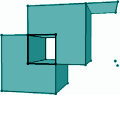
\includegraphics[width=12.0cm]{figs/teaser}}
%%     \caption{Demo application running on Windows. A polygon mesh is 
%%              subdivided using the quad-triangle subdivision 
%%              scheme~\cite{sl-qts-02}.}
%%     \label{fig:teaser}
%% \end{figure}



%% % open

%% Open source and contributions are welcome. 


%% % remainder

%% Section 2 describes how to declare a polyhedron, read a polygon mesh
%% from a file, and iterate over all facets for rendering. Example is
%% shown to enrich a polyhedron with extended primitives (normals,
%% colors, curvature tensors).

%% Section 3 illustrates how to write subdivision algorithms for meshes
%% (since they act on both connectivity and geometry, it is perfect for
%% our training purpose). Three approaches are shown. First one is sqrt3
%% subdivision using Euler operators. Second one uses the incremental
%% builder (originally designed for file IO) with a control mesh as
%% input. Third one offers a generic design for writing subdivision
%% algorithms.



%% % Andy

%% %program 1: rendering and file io of a default polyhedron 
%% %   context: a skeleton of a polyhedron program: declaration,
%% %initialization (inc. builder) and the rendering (iteration on facet and
%% %circulation of the facets)

%% %program 2: enriched polyhedron in program 1
%% %   context: extend a polyhedron: trait, item. hds? Use of the extended
%% %primitives.

%% %program 3: subdivision 1 (sqrt3)
%% %   context: refinement operators. Halfedge traversal (prev(), etc...) and
%% %circulators. Effect of connectivity edit on iterator and circulator.
%% %Maintain the correspondence after refinement.

%% %program 4: subdivision 2 (qt)
%% %   context: inc builder revisited.

%% %program 5: subdivisions (templated rules)
%% %   context: a generic design of subdivisions.

%% %program 2 is based on program 1 and program 3, 4, 5 are separate library
%% %functions called by program 2.

%% %The tutorial will walk though the programs. And a possible structure is
%% %sect 1: intro
%% %sect 2: program 1 & 2
%% %sect 3: program 3 & 4 & 5
%% %sect 4: conclusion 
        







